\chapter{Hardware di destinazione}
    
Come è stato scritto nell'introduzione la scheda \textit{Arduino Uno R3} è stata scelta per velocizzare lo sviluppo e per permettere al progetto di essere accessibile per un considerevole numero di utenti tenendo in considerazione le capacità e le competenze del segmento di pubblico al quale la scheda è rivolta.

\begin{figure}[b]
    \centering
    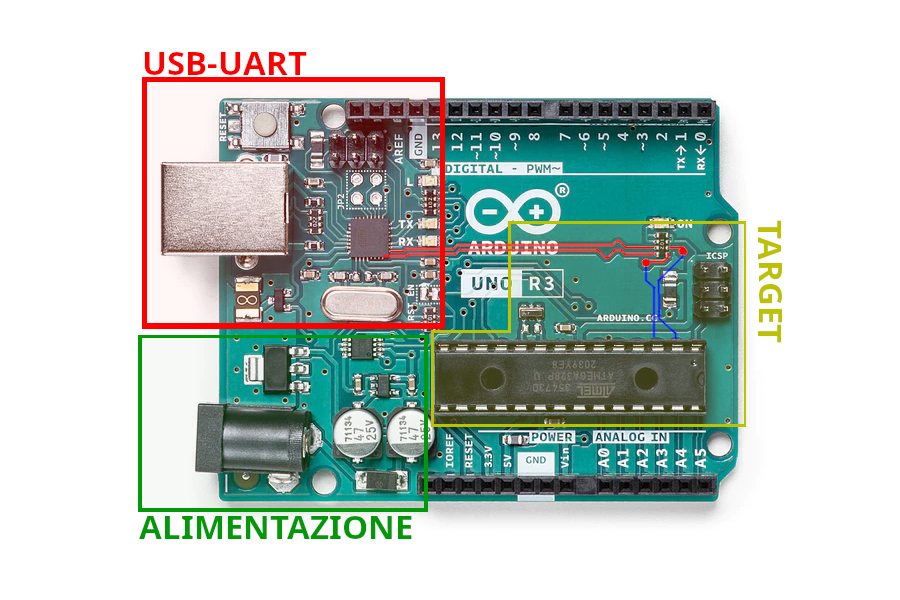
\includegraphics[width=.5\textwidth]{arduino-uno.png}
    \caption[]{Foto di una scheda Arduino Uno R3\cite{img:arduino-uno-r3}}\label{fig:arduino-uno-r3}
\end{figure}

la scheda (Figura~\ref{fig:arduino-uno-r3}) presenta una serie di connettori posti ai lati, collegati ai pin del controllore principale in centro, utili per interconnettere il dispositivo con i circuiti in sviluppo.
L'hardware addizionale presente sul lato sinistro --- invece --- permette di alimentare la scheda da una sorgente esterna non regolata tramite il connettore cilindrico nero e di collegare il controllore principale, tramite connessione seriale, a un computer tramite la porta USB presente in alto a sinistra.
È inoltre possibile effettuare il reset manuale del target tramite il pulsante presente vicino alla presa USB.\@

Il controllore presente al centro della scheda, in un involucro DIP-28\footnote{Dual in-line package, 28 pin}, è un ATMega328P-PU\cite{site:arduino-uno-doc}. È stato scelto un formato così ``datato'' per permettere all'utente di sostituire il chip in caso di guasto.

\section{La famiglia AVR}

Il controllore ATMega328P-PU presente sulla scheda di sviluppo è un membro della famiglia AVR di Atmel\cite{avr:m328p}.

Come è possibile identificare dalla figura~\ref{fig:avr-arch} l'architettura del processore della famiglia AVR è di tipo Harvard: È evidente la dicotomia tra memoria del programma (nell'immagine ``\textit{Flash Program Memory}''), SRAM e EEPROM\cite{harvard-arch}.

La suddivisione consente di ottimizzare separatamente le due diverse tecnologie di storge intrinsecamente diverse.

Come è possibile osservare, la grandezza del bus dati è di 8 bit, di conseguenza è possibile dedurre che l'intera architettura si basa sull'unità fondamentale del byte.

Vi è poi la totale assenza di pipelining essendo un processore a singolo ciclo. La maggior parte delle istruzioni, infatti, viene eseguita in un solo ciclo di clock\cite{avr:m328p} ad esclusione delle operazioni sulle memorie le quali ``stallano'' il processore per questioni di tempi di accesso/scrittura o di istruzioni che involvono dati di lunghezza maggiore di 8 bit.

\begin{figure}[t]
    \centering
    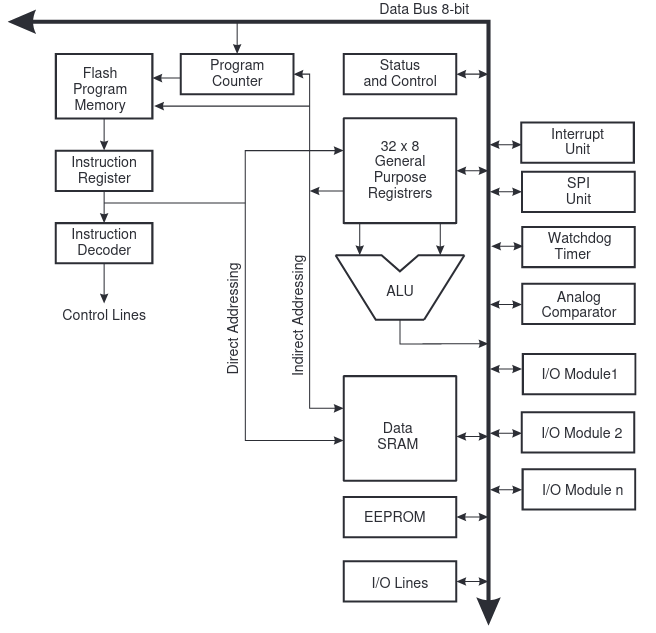
\includegraphics[width=.9\textwidth]{avr_arch.png}
    \caption[Immagine ottenuta dal documento~\cite{avr:m328p}, fig. 7-1]{Schema a blocchi dell'architettura AVR\cite{avr:m328p}}\label{fig:avr-arch}
\end{figure}

\subsection{Funzionalità avanzate}\label{ss:advanced-features}

Infine, per i micro controllori di fascia media, esiste la differenziazione tra codice di bootloader e codice eseguibile.

Il codice ``privilegiato'' è in grado di essere eseguito se si verificano determinati eventi, può essere protetto da sovrascrittura/lettura con criteri diversi dal codice dell'applicazione ed è in grado di riprogrammare la memoria dello stesso integrato mentre è in esecuzione (Read While Write)\cite{avr:m328p}.

\subsection{Memorie}

All'interno di un controllore della famiglia AVR, essendo un processore ad architettura harvard, è possibile trovare due diverse tipologie di memorie dedicate --- utili all'ottimizzazione di costi e funzionamento --- e una terza tipologia tipologia dedicata all'utilità e alla riduzione dei costi dell'hardware.

\subsubsection{Memoria FLASH}
La memoria flash è dedicata alla conservazione del codice eseguibile.
Dato l'utilizzo generale di sola lettura, essa si presenta come una memoria a lettura veloce, organizzata ad unità elementari di 16 bit e riprogrammabile a pagine.

La scelta di indicizzare a ``word'' è stata adottata in quanto la dimensione delle istruzioni dell'\textit{Instruction Set} è sempre di 16 bit oppure, in casi eccezionali, di 32 bit\cite{avr:isa}.

Si tratta poi di una memoria complessa: per i controllori avanzati, aventi il supporto al bootloader, essa è divisa in due sezioni le quali garantiscono la possibilità di differenziare i privilegi del codice presente nelle due sezioni come descritto nella sezione~\ref{ss:advanced-features}.

Essendo poi una memoria ``di programma'', essa non richiede prestazioni notevoli in scrittura: questa avviene quindi a blocchi di 512/1024byte (in funzione del controllore e della dimensione della memoria) e può essere eseguita in due diverse modalità:
\begin{itemize}
    \item ISP\footnote{In System Programming}: In questo caso il controllore è in modalità di programmazione ed esegue i comandi inoltrati da un programmatore esterno --- connesso tramite SPI\footnote{Serial Peripheral Interface} --- mentre la cpu è in stato di \textit{halt}.
    \item Self Programming: Grazie all'istruzione \texttt{spm} è possibile riprogrammare le pagine della memoria flash dall'interno del codice stesso\footnote{Nel caso in cui sia presente il supporto al bootloader, \texttt{spm} può essere eseguito solo se il program counter punta a tale regione.}.
\end{itemize}

\subsubsection{EEPROM}

La memoria EEPROM è considerata una memoria di utilità in quanto non necessariamente essenziale alla vita del codice in esecuzione. Essa permette di salvare dati in modo non volatile nell'eventualità di una mancanza di alimentazione.

Si tratta di una memoria ``lenta'' (tempi di programmazione di 3.3ms~\cite{avr:m328p}) ma in grado di essere letta e scritta con un'unità fondamentale di 8 bit.

Il vantaggio che si presenta con l'integrazione di tale memoria all'interno dell'integrato consiste nell'eliminazione di un ulteriore componente sul circuito stampato nel caso essa sia necessaria, oltre al non utilizzo di una periferica di comunicazione dedicata a tale scopo.

L'interazione con la memoria avviene tramite la scrittura e lettura di determinati registri (\texttt{EECR} \texttt{EEDR} \texttt{EEAR}, EEPROM Control, Data e Address Registers)\cite{avr:m328p}.

\subsubsection{SRAM}
La memoria SRAM è una delle maggiori costituenti della struttura dell'integrato.

Essa consiste nella principale memoria di elaborazione, ma la sua struttura è leggermente più complessa rispetto a quanto si possa trovare su un comune calcolatore.
Infatti l'architettura AVR utilizza in modo marcato il concetto di MMIO\footnote{Memory Mapped Input and Output}.

\begin{figure}[b]
    \centering
    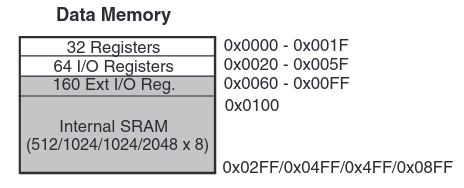
\includegraphics[width=.7\textwidth]{avr_sram_allocation.png}
    \caption[Immagine ottenuta dal documento~\cite{avr:m328p}, fig. 8-3]{Settorizzazione della memoria SRAM del controllore ATMega328P\cite{avr:m328p}}\label{fig:avr-sram-alloc}
\end{figure}

Come è possibile osservare dalla figura~\ref{fig:avr-sram-alloc} i primi 128 byte della memoria SRAM sono in realtà registri di uso generale (\texttt{r0}-\texttt{r31}) o registri di controllo delle periferiche.
La scrittura di tali locazioni di memoria causa effetti collaterali in funzione della periferica alla quale è associata.

È inoltre necessario notare dalla figura~\ref{fig:avr-sram-alloc} come le istruzioni di accesso alla ram impieghino due cicli di clock:l'indicizzazione della ram è effettuata tramite un indirizzamento di 16 bit, il quale rende necessario l'utilizzo congiunto di due registri (r26-r27, r28-r29, r30-r31). 

Questa operazione infatti consente di calcolare l'indirizzo al quale effettuare l'operazione incrementando, decrementando oppure lasciando invariata la coppia di registri di indicizzazione pre o post esecuzione.

\begin{figure}[t]
    \centering
    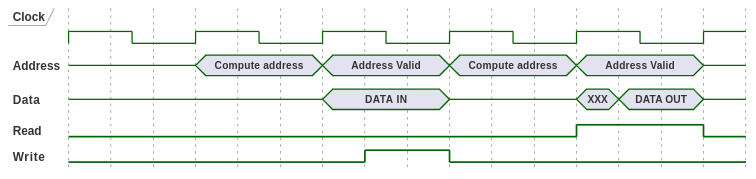
\includegraphics[width=.9\textwidth]{sram-access-timings.png}
    \caption[Immagine rielaborata a partire dalla fig. 8-4 del documento~\cite{avr:m328p}]{Sequenze di accesso in lettura e scrittura della memoria SRAM\cite{avr:m328p}}\label{fig:avr-sram-timings}
\end{figure}

in particolare, un uso comune delle istruzioni di accesso alla memoria viene mostrato dal listato~\ref{lst:store-example}, riga 7

\begin{lstlisting}[language=AVR, caption={Esempio di utilizzo dell'istruzione \texttt{st}}, label=lst:store-example]
    ldi r24, 0xFF ;Salva la costante 0xFF nel registro r24
    eor r0, r0 ;Salva la costante 0x00 nel registro r0
    eor r26, r26 ;Azzera il contenuto di r26 (XL)
    eor r27, r27 ;Azzera il contenuto di r27 (XH)
loop:
    st r24, X+ ;SRAM[r27:r26] = r24
    dec r24 ;r24--
    cpse r24, r0 ;if(r24 == 0) goto hold
    rjmp loop ;else goto loop
hold:
    rjmp hold ;goto hold

\end{lstlisting}

In particoare il codice presentato dal listato~\ref{lst:store-example}, dopo una breve fase di inizializzazione (linee 1-4) dove vengono azzerati i registri r0, r26 e r27 (dove gli ultimi due elencati vengono definiti nel codice dal meta-registro X), definisce un ciclo dove viene salvato il contenuto di r24 all'indirizzo puntato dal registro X con successivo incremento, seguito dall'istruzione \texttt{cpse}\footnote{Compare and Skip if Equal} la quale compara rispetto alla costante 0 il valore di r24 una volta decrementato. Nel caso in cui la comparazione risulti veritiera, viene incrementato il program counter di due word, terminando quindi l'esecuzione nel ciclo di hold.

\section{Il protocollo DebugWire}

Parte fondamentale del core avr, omessa dal diagramma in figura~\ref{fig:avr-arch}, è il sistema di debugging on chip ``\textit{DebugWire}''.

Esso permette, tramite un tool esterno collegato all'integrato, di stallare la cpu e leggere e scrivere le memorie e i registri.\cite{avr:m328p}

Affinchè le funzionalità di debugging siano disponibili, è necessario abilitare la periferica DebugWire tramite i bit di configurazione al momento della programmazione del dispositivo.

\subsection{Interfaccia fisica}

L'interfacciamento fisico tra controllore e dispositivo esterno avviene tramite una sola connessione al pin di reset dell'integrato \textit{target}.

Il fatto che l'interfaccia di debug sia collocata sul pin di reset comporta che, una volta abilitata la periferica DebugWire, non sia più possibile resettare il dispositivo o programmarlo tramite interfaccia ISP\cite{avr:appnote:isp}\cite{avr:m328p}.

La comunicazione tra programmatore e target è di tipo seriale e half duplex data la natura della connessione. In particolare il protocollo utilizzato è una derivazione di una seriale UART su un bus open collector, come è osservabile dalla figura~\ref{fig:dw-schematic}\cite{site:dw-reverse-engeneering}.

\begin{figure}[t]
    \centering
    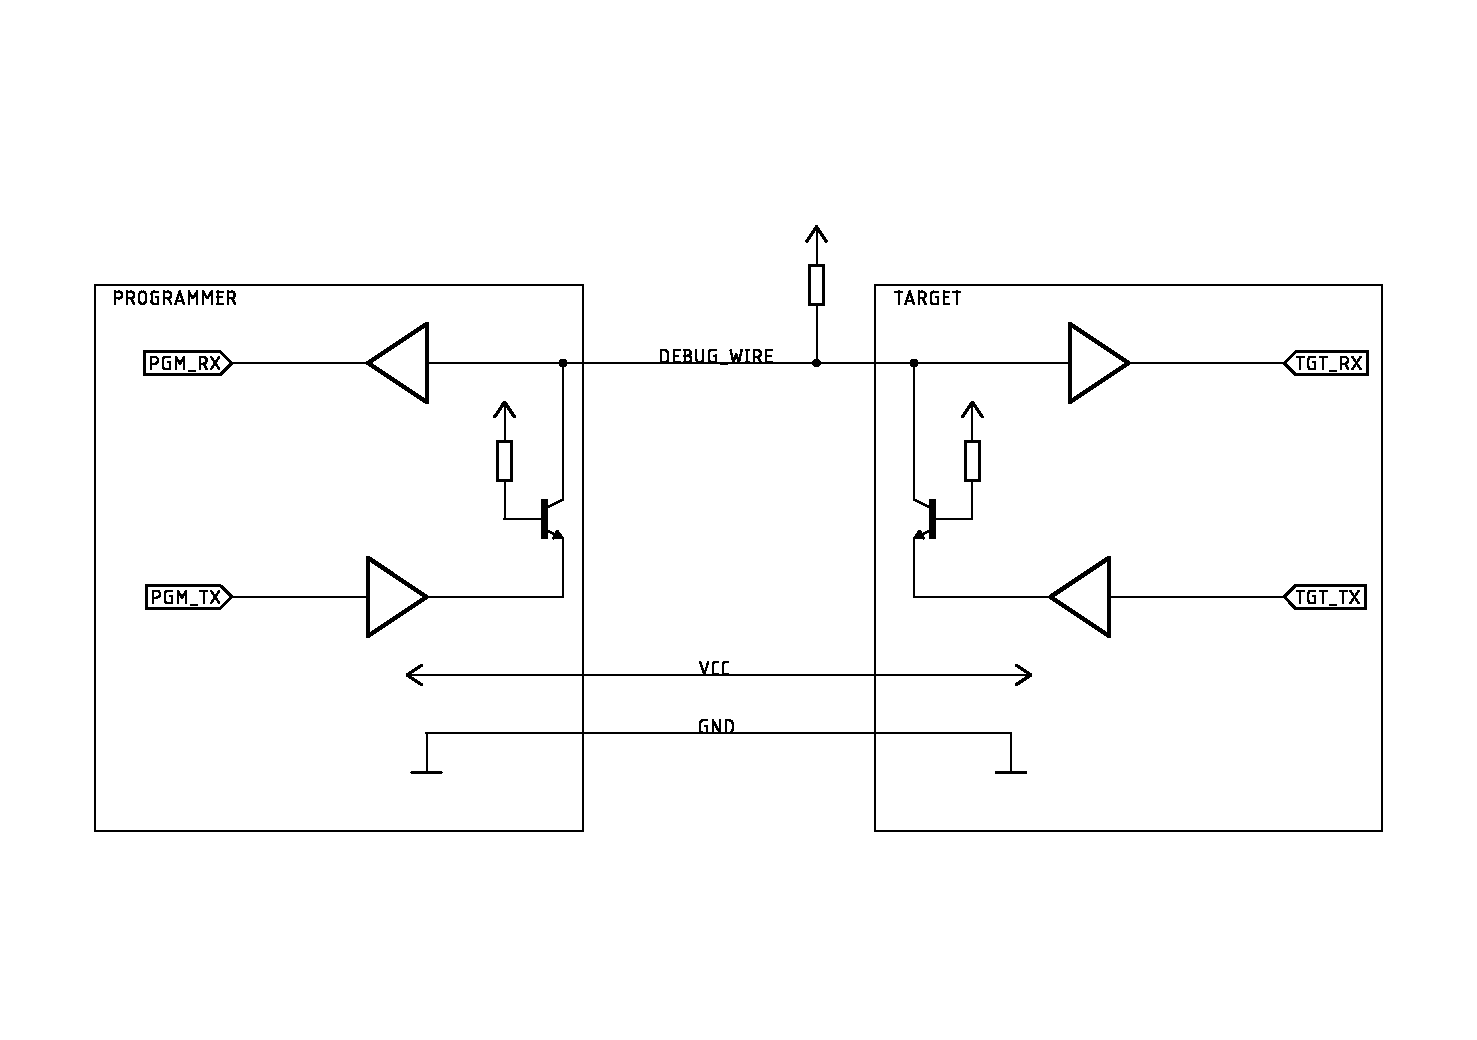
\includegraphics[width=\textwidth]{dw-schematic.pdf}
    \caption[]{Schema concettuale del funzionamento dell'interconnessione tra programmatore e controllore target per il protocollo DebugWire}\label{fig:dw-schematic}
\end{figure}

\subsubsection{Protocollo UART}

Il protocollo UART è un metodo di trasmissione punto-punto digitale seriale asincrono che generalmente lavora su due connessioni tra i due attori della comunicazione. Le due linee rimangono a livello logico 1 quando non c'è attività.

Le due linee prendono il nome di ``tx'' e ``rx'', in funzione dell'utilizzo che la periferica master ne fa: è necessario notare come le due linee vengano ``incrociate'' in modo tale da far sì che il pin di trasmissione di un attore vada a collegarsi con il pin di ricezione della controparte.

Essendo un protocollo asincrono, ovvero vi è assenza di una linea di sincronizzazione (clock), le due parti della comunicazione devono conoscere a priori la velocità attesa sulle linee.

La trasmissione inizia con un periodo di livello logico 0, in modo che sia possibile identificare l'inizio della trasmissione di un byte rilevando il fronte di transizione da livello logico 1 a livello logico 0.

Durante questo tempo di bit dove la linea di trasmissione è a livello logico 0 è dunque possibile inizializzare l'hardware e sincronizzare le sorgenti di clock per la ricezione. In seguito al bit di inizio (Start Bit) si susseguono, i bit del dato, dal meno significativo al più significativo, con periodo pari al tempo di bit stesso. In funzione della specifica del protocollo possono essere inviate unità di dati fondamentali di dimensione da 5 a 8 bit nota a priori.

A seguito dei bit di dati viene quindi inviato opzionalmente un bit di parità per garantire l'integrità dei dati e successivamente la linea viene posta a livello logico 1 per uno o due periodi di bit, permettendo al ricevitore di eseguire operazioni e resettare la macchina a stati per la ricezione.\cite{site:rs-uart}

Essendo un sistema asincrono è opportuno ipotizzare il non allineamento delle frequenze di invio e campionamento: In tal caso una desincronizzazione può essere tollerata se entro il limite dato dall'equazione~\ref{eq:uart-max-delay}
\begin{equation}\label{eq:uart-max-delay}
    t_{delay_{\max}} = \frac{1}{2}N_{bits-per-symbol}t_{bit}    
\end{equation}
dove \(N_{bits-per-symbol}\) è il numero di bit contenuti nel simbolo inviato e \(t_{bit}\) è il tempo per bit. Questo comportamento può essere notato dalla figura~\ref{fig:uart-sync}, dove vengono rappresentati il caso ideale e il caso di desincronizzazione massima. In ogni caso si ha che il campionamento avviene all'interno del bit in invio.

\afterpage{
    \begin{figure}[h]
        \centering
        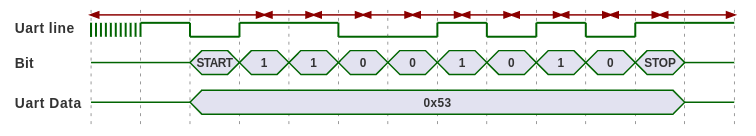
\includegraphics[width=.8\textwidth]{uart-sync.png}\\
        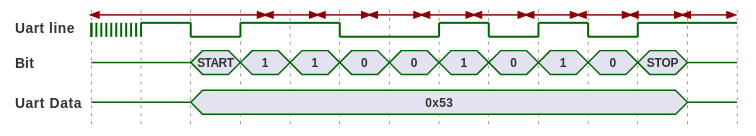
\includegraphics[width=.8\textwidth]{uart-unsync.png}
        \caption[]{I diagrammi di sequenza dimostrano che, anche in caso di non sincronizzazione delle frequenze di invio e ricezione viene mantenuta l'integrità dei dati trasmessi. Viene mostrata una comunicazione seriale 8N1\footnote{Definizione della configurazione di una linea seriale. Essa è composta da tre caratteri: <Numero di bit dati><Tipo di parità ([N]one, [O]dd, [E]ven, [M]ark, [S]pace)><Numero di Stop bits>}}\label{fig:uart-sync}
    \end{figure}
}

La motivazione per cui il campionamento avviene a metà del tempo di bit è data dal fatto che la desincronizzazione possa essere causata da una frequenza più alta o più bassa, per cui vale la relazione descritta dall'equazione~\ref{eq:uart-period-receive-delay}
\begin{equation}\label{eq:uart-period-receive-delay}
     t_{bit_{recv}} = t_{bit_{snd}} \pm t_{delay_{\max}}
\end{equation}

Infine, se la velocità di trasmissione fosse misurata in \textit{bit per secondo}, secondo la formula \(v_{uart} = \frac{1}{t_{bit}}\), essa non sarebbe veritiera e porterebbe confusione, in quanto la formula sopra enunciata includa nel conteggio dei bit trasmessi anche i bit di controllo (Start e Stop bit) i quali non contribuiscono all'informazione inviata. Di conseguenza è opportuno definire la velocità di trasmissione della linea seriale come il numero di simboli trasmessi per secondo. Questa definizione differisce dalla prima un quanto il simbolo è composto da un numero di bit non necessariamente pari a 8.

È possibile determinare la velocità in baud a partire dal bitrate e dalla configurazione della linea UART secondo la relazione~\ref{eq:baud-from-bit-rate}\cite{site:baud}:
\begin{equation}\label{eq:baud-from-bit-rate}
    v_{tx_{baud}} = \frac{1}{t_{bit}(N_{databits} + N_{parity} + 2)}
\end{equation}

Da quanto è possibile dedurre dall'equazione~\ref{eq:baud-from-bit-rate}, è possibile verificare come l'effettivo bit rate di trasmissione della linea UART differisca di un fattore di \(\frac{N_{databits}}{N_{databits} + N_{parity} + 2}\) rispetto al bitrate grezzo di trasmissione \(v_{uart}\)

\subsection{Funzionamento}

Tutte le comunicazioni che avvengono sul bus DebugWire non hanno alcun tipo di verifica dell'integrità del dato (CRC). La comunicazione può avvenire in qualsiasi momento.

In particolare il reset della comunicazione tra target e prgogrammatore/debugger avviene mediante l'invio di un BREAK\footnote{La linea viene posta a livello logico 0 per più di 9 tempi di bit} sulla linea.
Ogni qualvolta sia rilevato un errore (per esempio viene ricevuto un byte inatteso o un comando non noto), il primo attore che rileva l'errore invierà un BREAK che causerà il reset della controparte.

Ciò è possibile perchè la connessione è un bus open collector: il conflitto di accesso avviene solo ponendo la linea a livello logico 0 e non comporta cortocircuitazioni di qualsiasi genere. Il conflitto viene rilevato quando un attore riceve un dato diverso da quanto inviato (in particolare quando l'eattore riceve un bit pari a 0 quando sta inviando un bit di valore 1).

La velocità di comunicazione è invece definita in funzione della frequenza della cpu del target. Nell'hardware della periferica è presente un prescaler (il cui valore di default è di 128) e la velocità di comunicazione viene stabilita come \[v_{com} (BAUD) = \frac{f_{cpu} (Hz)}{prescaler}\]

Ad ogni reset della comunicazione il prescaler viene resettato al valore inizale (128).

In risposta ad un BREAK il target risponderà sempre con l'invio di un valore noto (0x55), facendo sì che a livello fisico sia inviata un'onda quadra con frequenza \(v_{com}\)\cite{site:dw-reverse-engeneering} (si veda figura~\ref{fig:dw-timings})

\begin{figure}[h]
    \centering
    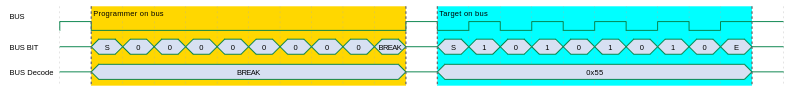
\includegraphics[width=\textwidth]{dw-break-timing.png}
    \caption[]{Diagramma delle tempistiche del bus DebugWire durante il reset della trasmissione}\label{fig:dw-timings}
\end{figure}

È dunque possibile definire un algoritmo per l'inizializzazione della sessione in modo che la frequenza della trasmissione venga dedotta dalla risposta del target invece che essere nota a priori:
\begin{enumerate}
    \item Preparazione dell'hardware e inizializzazione strutture dati
    \item Invio di un break dalla durata di 100ms. La durata viene stabilita in funzione della frequenza di trasmissione ragionevolmente più bassa possibile: Considerando che la famiglia AVR integra negli integrati un oscillatore RC a 128kHz usato comunemente per operazioni ``low power'', ipotizzando che sia abilitata la funzionalità di divisione del clock per un fattore di 8\cite{avr:m328p}, si ottiene una frequenza del core di 16kHz. Ponendo quindi il prescaler di comunicazione DebugWire a 128 otteniamo una frequenza di trasmissione di 125Hz, ovvero 8ms per bit. Infine, sapendo che il tempo di break consiste in almeno 10 bit trasmessi a 0, si ottiene un tempo minimo di break di 80ms, arrotondato a 100ms
    \item Attesa del primo fronte di trasizione da livello logico 1 a livello logico 0
    \item Attesa del successivo fronte di transizione da livello logico 0 a livello logico 1 (calcolando il tempo intercorso tra i due fronti)
\end{enumerate}

A questo punto è possibile trovare la frequenza di bit dalla quale ricavare il baudrate.

\subsection{Comandi e features}

Una volta che la cpu del controllore target è in stato \textit{halt} è possibile interagire con la periferica DebugWire per eseguire le operazioni di debug. A seguito di un BREAK e successiva risposta è possibile interpellare il controllore con i comandi descritti di seguito.

Vi sono due classi di comandi: Comandi basilari e comandi composti.
I primi sono comandi che svolgono azioni semplici e definite staticamente, quali la scrittura del Program Counter, Instruction register, scrittura del registro di breakpoint hardware e configurazione di flag e comunicazione. Tramite questi comandi è possibile definire i limiti di scrittura/lettura delle memorie e eseguire istruzioni.

I comandi disponibili per l'interazione con il microcontrollore target tramite DebugWire sono limitati e appartengono a quattro categorie: \textit{Communication Settings}, \textit{Flag Setting},\textit{Program Flow Control} e \textit{Memory R/W}.

\subsubsection{Communication Settings}

Questi comandi vengono utilizzati per modificare il valore del prescaler di comunicazione in modo da modificare la velocità di trasmissione. Sono comandi particolarmente utili nel debugging di controllori a bassa frequenza (128kHz).

Non vi è una logica nota nell'assegnazione del comando al corrispondente valore del prescaler: si rende necessaria una tabella di associazione come riportato dalla tabella~\ref{tab:dw-presc-settings}

\begin{table}[h]
    \centering
    \begin{tabular}{ c c c }
        \textbf{Comando} & \textbf{Valore del prescaler} & \textbf{Bitrate a 16MHz} \\
        \hline
        0x83 & 128 & 125kbps \\
        0x82 & 64 & 254kbps \\
        0x81 & 32 & 500kbps \\
        0x80 & 16 & 1Mbps \\
        0xA0 & 8 & 2Mbps \\
        0xA1 & 4 & 4Mbps \\
        0xA2 & 2 & 8Mbps \\
        0xA3 & 1 & 16Mbps \\
        \hline
    \end{tabular}
    \caption[]{Tabella descrittiva dei comandi per la modifica del prescaler di trasmissione della periferica di debug del controllore target\cite{site:dw-reverse-engeneering}}\label{tab:dw-presc-settings}
\end{table}

Una volta inviato il comando di configurazione del prescaler il controllore si adatterà alla velocità richiesta e risponderà con il valore \texttt{0x55} inviato alla nuova frequenza. Questo valore può essere usato per settare adattivamente la frequenza del programmatore oppure per verificare che le impostazioni siano corrette.

\subsubsection{Flag Setting}

È necessario configurare lo stato della periferica prima di eseguire effettivamente le operazioni che sono state preparate. Possiamo chiamare questo stato ``Contesto di esecuzione'' in quanto la stessa configurazione dell'hardware permette di eseguire diverse azioni in funzione del contesto che viene configurato.

I contesti disponibili sono elencati nella tabella~\ref{tab:dw-contexts}.

\begin{table}[h]
    \centering
    \begin{tabular}{ c l }
        \textbf{Comando dW} & \textbf{Contesto} \\
        \hline
        0x60 & Ripresa dell'esecuzione\\
        0x61 & Ripresa dell'esecuzione fino all'indirizzo HWBP\\
        0x64 & Lettura/Scrittura memoria Flash\\
        0x66 & Lettura/Scrittura della SRAM\\
        0x79 & Riprese dell'esecuzione usando l'istruzione caricata\\
        0x7A & Single Step\\
        \hline
    \end{tabular}
    \caption[]{Tabella descrittiva dei contesti di esecuzione DebugWire\cite{site:dw-reverse-engeneering}}\label{tab:dw-contexts}
\end{table}

È possibile inoltre modificare i contesti ponendo il valore del bit 5 a zero per permettere alle periferiche di temporizzazione (timers) di continuare il conteggio durante lo stepping.

\subsubsection{Program Flow Control}

Questi comandi sono utilizzati per confermare le operazioni da eseguire.

Esistono comandi di ``GO'' per le varie operazioni composite quali la lettura e scrittura della memoria SRAM (0x20 per indirizzi multipli, 0x21 per un indirizzo singolo), esecuzione di un'istruzione precedentemente caricata in IR senza incrementare il program counter (0x23), ripresa dell'esecuzione (0x30) o single stepping (0x31).

Se il bit 5 è settato allora il target effettuerà il reset della sessione inviando un BREAK seguito da 0x55 al termine dell'esecuzione.

\subsubsection{Memory R/W}

Questi sono i comandi fondamentali per la scrittura e lettura dei registri PC, IR, HWBP e SIGNATURE (sola lettura).

Questi registri possono essere trattati relativamente alla loro funzione oppure possono essere visti come parametri di configurazione per le operazioni composite descritte in seguito.

I registri di configurazione sono mappati ad un indice come descritto dalla tabella\ref{tab:dw-regs-idx}.

\begin{table}[h]
    \centering
    \begin{tabular}{ c l }
        \textbf{Indice} & \textbf{Registro associato} \\
        \hline
        0 & Program Counter (PC)\\
        1 & Hardware Breakpoint (HWBP)\\
        2 & Instruction Register IR\\
        3 & DW Signature register\\
        \hline
    \end{tabular}
    \caption[]{Tabella descrittiva dell'associazione degli indici ai registri elementari\cite{site:dw-reverse-engeneering}}\label{tab:dw-regs-idx}
\end{table}

Le operazioni di lettura e scrittura dei registri avvengono mediante l'invio di pacchetti come definito dalle figure~\ref{fig:dw-reg-wrt}~e~\ref{fig:dw-reg-rd}

\begin{figure}[h]

    \centering
    \begin{bytefield}[endianness=big,bitwidth=1em]{24}
        \bitheader{0-23}\\
        \bitbox{4}{0xD} & \bitbox{4}{idx} & \bitbox{16}{data}\\
    \end{bytefield}

    \caption[]{Pacchetto di scrittura di un registro elementare. Nessuna risposta da parte del target}\label{fig:dw-reg-wrt}
\end{figure}


\begin{figure}[h]

    \centering

    \begin{lrbox}{\bytefieldbox}
        \begin{bytefield}[endianness=big,bitwidth=1em]{8}
            \bitheader{0-7}\\
            \bitbox{4}{0xF} & \bitbox{4}{idx} \\
        \end{bytefield}
    \end{lrbox}
    \subfloat[]{\usebox{\bytefieldbox}}

    \begin{lrbox}{\bytefieldbox}
        \begin{bytefield}[endianness=big,bitwidth=1em]{16}
            \bitheader{0-15}\\
            \bitbox{16}{data}\\
        \end{bytefield}
    \end{lrbox}
    \subfloat[]{\usebox{\bytefieldbox}}


    \caption[]{Pacchetto di lettura di un registro elementare (a) e successiva risposta (b)}\label{fig:dw-reg-rd}
\end{figure}

\subsubsection{Comandi compositi}

DebugWire permette di leggere e scrivere la memoria SRAM mediante una combinazione di comandi elementari.
Grazie a questa funzionalità è possibile leggere e scrivere sia la memoria dati che i registri di configurazione delle periferiche e i registri ``general purpose'' come viene evidenziato dalla figura~\ref{fig:avr-sram-alloc}.

L'algoritmo per la scrittura dei registri (r0-r31) consiste in quanto segue\cite{site:dw-reverse-engeneering}:
\begin{enumerate}
    \item Context: SRAM R/W
    \item Scrittura del registro iniziale nel registro PC
    \item Scrittura del registro finale nel registro HWBP
    \item Selezione modalità (Comando C2 seguito dall'indice dell'operazione come descritto nella tabella~\ref{tab:dw-ops})
    \item GO SRAM R/W
    \item (Se scrittura) Invio dei byte da scrivere.\\(Se lettura) ricezione dei byte letti.
\end{enumerate}

\begin{table}[t]
    \centering
    \begin{tabular}{ c l }
        \textbf{Indice} & \textbf{Modalità} \\
        \hline
        0 & Lettura memoria SRAM\\
        1 & Lettura registri \\
        2 & Lettura memoria Flash\\
        4 & Scrittura memoria SRAM\\
        5 & Scrittura registri\\
        \hline
    \end{tabular}
    \caption[]{Tabella descrittiva dell'associazione degli indici alle modalità di operazione sulle memorie\cite{site:dw-reverse-engeneering}}\label{tab:dw-ops}
\end{table}

Di seguito, alla figura~\ref{fig:dw-reg-rw-com}, viene riporatta la traccia di comunicazione per questo algoritmo.

Analogamente è possibile leggere e scrivere la memoria SRAM e leggere la memoria FLASH con il seguente algoritmo:
\begin{enumerate}
    \item Scrittura dell'indirizzo di partenza nella coppia di registri \texttt{r30 - r31}
    \item Scrittura del registro PC al valore 0x0000 se lettura o 0x0001 se scrittura
    \item Scrittura del doppio della lunghezza dei dati (+1 se in scrittura) da leggere/scrivere registro HWBP
    \item Selezione modalità
    \item GO con appropriata modalità.
\end{enumerate}

Di seguito, alla figura~\ref{fig:dw-mem-rw-com}, viene riporatta la traccia di comunicazione per questo algoritmo.

Inoltre è possibile eseguire direttamente un'istruzione senza scriverla nella memoria Flash. In questo caso è sufficiente scrivere nel registro IR l'opcode dell'operazione ed eseguire il comando di flow control (0x23 o 0x33). Si noti che non è possibile eseguire istruzioni di 32 bit.

\begin{figure}[p]

    \centering
    \begin{bytefield}[endianness=big,bitwidth=1em]{32}
        \bitheader{0-31}\\
        \bitbox{8}{CNTX\_SRAM} & \bitbox{8}{0xD0} & \bitbox{16}{start\_reg} \\
        \bitbox{8}{0xD1} & \bitbox{16}{end\_reg + 1} & \bitbox{8}{0xC2} \\
        \bitbox{8}{MOD: 0x00/0x05} & \bitbox{8}{GO MEM}
    \end{bytefield}

    \caption[]{Comunicazione inviata dal debugger per leggere/scrivere i registri. In caso di scrittura viene seguita da (end\_reg - start\_reg) byte, altrimenti la stessa quantità di byte viene ricevuta.}\label{fig:dw-reg-rw-com}
\end{figure}

\begin{figure}[p]

    \centering
    \begin{bytefield}[endianness=big,bitwidth=1em]{32}
        \bitheader{0-31}\\
        \bitbox{8}{CNTX\_SRAM} & \bitbox{24}{0xD0001E} \\
        \bitbox{24}{0xD10020} & \bitbox{8}{0xC2} \\
        \bitbox{8}{0x05} & \bitbox{8}{0x20} & \bitbox{16}{addr\_start} \\
        \bitbox{8}{0xC2} & \bitbox{8}{0x04/0x00/0x01} & \bitbox{16}{0xD000} \\
        \bitbox{8}{0x00/0x01} & \bitbox{8}{0xD1} & \bitbox{16}{len * 2 (+1 if wrt)}\\
        \bitbox{8}{GO MEM}
    \end{bytefield}

    \caption[]{Comunicazione inviata dal debugger per leggere/scrivere le memorie. In caso di scrittura viene seguita da \textit{len} byte, altrimenti la stessa quantità di byte viene ricevuta.}\label{fig:dw-mem-rw-com}
\end{figure}

Si noti come i valori dei registri \texttt{Z, PC, HWBP e IR} venga modificata da queste operazioni. Ciò rende necessaria una procedura di salvataggio e ripristino prima di riprendere l'eventuale esecuzione del codice sul dispositivo \textit{target}.